\documentclass[12pt, a4paper]{article} \pagenumbering{gobble}
\usepackage{gantt} \usepackage{pdflscape} \usepackage{parskip}
\usepackage{afterpage} \usepackage{pbox}
\usepackage[margin=1in]{geometry} \usepackage{multirow,tabularx}
\usepackage{wrapfig}
\usepackage{graphicx}
\usepackage{listings}
\usepackage[dvipsnames]{xcolor}
\graphicspath{ {images/} }
\pagenumbering{arabic}
\newcolumntype{Y}{>{\centering\arraybackslash}X}
\renewcommand{\arraystretch}{2}
\definecolor{new-blue}{RGB}{51,153,255}

\begin{document}
  \begin{titlepage}
    \centering
    {\scshape\Large Izmir Institute of Technology\par}
    {\scshape\large Department of Computer Engineering\par}
    {CENG415 Senior Design Project & Seminar 1\par}
    \vspace{2.5cm}
	  {\huge re\sqrt{ision}\par}
	  \vspace{1cm}
	  {\Large Renderscript for Computer Vision\par}
	\vspace{2cm}
	{\Large An{\i}l Can Ayd{\i}n, Onur Temizkan, Ula\c{s} Akdeniz\par}
  {\itshape180201060, 180201004, 180201063\par}
	\vfill
	supervised by\par
	\large{Asst. Prof. Dr.~Mustafa \textsc{\"{O}zuysal}}

	\vfill

% Bottom of the page
	{\large \today\par}
  \end{titlepage}
  \newpage
  \tableofcontents

\newpage
\begin{section}{Description of the Work}
\paragraph{}{%
  Computer vision applications need parallel computation to perform in reasonable response time.
  In order to satisfy that performance, developers use libraries like OpenCL and CUDA which move the computation
  load to GPU. However high performance GPU intensive computation on Android platform is a tough issue because
  of hardware dependencies and incompatibilities of libraries. For instance OpenCL GPU computation library is not
  supported on all Android devices. So, creating hardware independent applications using OpenCL is simply impossible.
  Because of those restrictions mentioned above, Renderscript computation module is presented by Google in 2011 \cite{renderscript_release}.
  It is a hardware-independent computation engine that operates at the native level \cite{renderscript_api}. But there is no vision library
  written in Renderscript.
}
\paragraph{}{%
  reVision is an open source, Renderscript powered computer vision library that can operate on all Android devices.
  It contains ready to use computer vision algorithm implementations with their sample applications. The vision
  algorithms are implemented in Renderscript. Also all Renderscript parts have their own Java parts for outer
  communication with Android platform.
}
\paragraph{}{Response times of reVision modules are small enough to process video streams in real time with minimum data loss. It also can be used in non-blocking way to not affect the other functionalities of client applications.}
\end{section}

\newpage

\begin{section}{Project Management}
  \begin{subsection}{Overall Strategy}
    \paragraph{}{reVision's iterative development process consists of project management and planning, requirement analysis, implementation and testing. Each iteration results in at least one new module with its sample application.}\\ \\
    Summary of an iteration is described below.
    \paragraph{Planning:}{The scope of the module to be written, desired specs and details are discussed.}
    \paragraph{Requirement Analysis:}{The output of the module, needed arguments and optional specs are discussed.}
    \paragraph{Implementation:}{The module and its sample application is implemented.
    \begin{itemize}
      \item Modules are main objectives of the every iteration.
      \item Proceed every iteration with phases such as: Design, Implement, Test and Evaluate.
    \end{itemize}}
    \paragraph{Testing:}{The module and the sample application are validated via unit tests.}
  \end{subsection}

  \newpage

  \begin{subsection}{Gantt Chart}
  \vspace*{\fill}
  \begin{centering}
  \scalebox{0.7}{
  \begin{gantt}[xunitlength=0.5cm,fontsize=\small,titlefontsize=\small,drawledgerline=true]{25}{32}
    \begin{ganttitle}
      \titleelement{October}{4}
      \titleelement{November}{4}
      \titleelement{December}{4}
      \titleelement{January}{4}
      \titleelement{February}{4}
      \titleelement{March}{4}
      \titleelement{April}{4}
      \titleelement{May}{4}

    \end{ganttitle}
    \begin{ganttitle}
      \numtitle{3}{1}{4}{2}
      \numtitle{1}{1}{4}{1}
      \numtitle{1}{1}{4}{1}
      \numtitle{1}{1}{4}{1}
      \numtitle{1}{1}{4}{1}
      \numtitle{1}{1}{4}{1}
      \numtitle{1}{1}{4}{1}
      \numtitle{1}{1}{4}{1}
    \end{ganttitle}
    \ganttbar[color=purple]{\textbf{Software Development}}{0}{32}
    \ganttbar[color=red]{\textbf{Research / Requirement Analysis}}{0}{12}
    \ganttbar[color=purple]{12.10.15 - 04.01.16}{0}{0}
    \ganttbar[color=red]{\textbf{Design}}{10}{2}
    \ganttbar[color=purple]{14.12.15 - 04.01.16}{0}{0}
    \ganttbar[pattern=crosshatch,color=green]{\textbf{Data Model Design}}{10}{1}
    \ganttbar[color=purple]{14.12.15 - 21.12.15}{0}{0}
    \ganttbar[pattern=crosshatch,color=green]{\textbf{Domain Model Design}}{11}{1}
    \ganttbar[color=purple]{21.12.15 - 04.01.16}{0}{0}
    \ganttbar[color=red]{\textbf{Implementation}}{12}{20}
    \ganttbar[color=purple]{04.01.16 - 30.05.16}{0}{0}
    \ganttbar[pattern=crosshatch,color=green]{\textbf{Filter Module}}{12}{3}
    \ganttbar[color=purple]{04.01.16 - 25.01.16}{0}{0}
    \ganttbar[pattern=crosshatch,color=green]{\textbf{Feature Module}}{14}{16}
    \ganttbar[color=purple]{11.01.16 - 16.05.16}{0}{0}
    \ganttbar[pattern=crosshatch,color=green]{\textbf{Data Module}}{15}{3}
    \ganttbar[color=purple]{19.01.16 - 09.02.16}{0}{0}
    \ganttbar[pattern=crosshatch,color=green]{\textbf{Async Module}}{20}{1}
    \ganttbar[color=purple]{15.02.16 - 07.04.16}{0}{0}
    \ganttbar[pattern=crosshatch,color=green]{\textbf{Samples}}{29}{2}
    \ganttbar[color=purple]{09.05.16 - 23.05.16}{0}{0}
    \ganttbar[pattern=crosshatch,color=green]{\textbf{Test}}{31}{1}
    \ganttbar[color=purple]{23.05.16 - 30.05.16}{0}{0}
  \end{gantt}
  }
  \end{centering}
  \vspace*{\fill}
\end{subsection}

\begin{landscape}% Landscape page
\subsection{Detailed Work Description}
  \subsubsection{Work Package List}
  \scalebox{0.7}{
   \begin{tabularx}{85em}{|*{8}{Y|}}
     \hline
       \textbf{Work Package No} & \textbf{Work Package Title} & \textbf{Type of Activity}\footnotemark[1] & \textbf{Lead Participant No} & \textbf{Lead Participant Short Name} & \textbf{Person weeks}\footnotemark[2] & \textbf{Start Month} & \textbf{End Month} \\
       \hline
       WP-1 & Research and Requirement Analysis & MGT & 1-2-3 & AA-OT-UA & 13 & 1 & 4 \\
       \hline
       WP-2.1 & Data Model Design & SUPP & 1-2-3 & AA-OT-UA & 1 & 3 & 3 \\
       \hline
       WP-2.2 & Domain Model Design & SUPP & 1-2-3 & AA-OT-UA & 2 & 3 & 4 \\
       \hline
       WP-3.1 & Filter Module & SUPP & 2 & OT & 3 & 4 & 4 \\
       \hline
       WP-3.2 & Feature Module & SUPP & 1-2-3 & AA-OT-UA & 18 & 4 & 8 \\
       \hline
       WP-3.3 & Data Module & SUPP & 1 & AA & 3 & 4 & 5 \\
       \hline
       WP-3.4 & Async Module & SUPP & 3 & UA & 3 & 5 & 6 \\
       \hline
       WP-3.5 & Samples & SUPP & 1-2-3 & AA-OT-UA & 2 & 8 & 8 \\
       \hline
       WP-4 & Testing & MGT & 1-2-3 & AA-OT-UA & 1 & 8 & 8 \\
       \hline
        \multicolumn{5}{|c|}{\textbf{TOTAL}} & \textbf{46} & & \\
        \hline
   \end{tabularx}
 }
\footnotetext[1]{\textbf{SUPP} stands for Support activities; \textbf{MGT} stands for Management of the consortium.}
\footnotetext[2]{The total number of person-weeks allocated to each work package.}
\end{landscape}
\subsubsection{Deliverable List}
    \begin{tabularx}{\textwidth}{|*{6}{Y|}}
        \hline
      \textbf{Deliverable No} & \textbf{Deliverable Name} & \textbf{WP No} & \textbf{Nature}\footnote{\textbf{R} = Report, \textbf{P} = Prototype, \textbf{D} = Demonstrator} & \textbf{Dissemination Level}\footnote{\textbf{PU} = Public, \textbf{CO} = Confidential, only for members of the consortium(including the Commission Services)} & \textbf{Delivery Date} \\
      \hline
        D-1 & Requirement Design Documents & WP-1 & R & CO & 24.12.2016 \\
        \hline
        D-2.1 & Data Model Design & WP-2.1 & R & CO & 21.12.2016 \\
        \hline
        D-2.2 & Domain Model Design & WP-2.2 & R & CO & 04.01.2016 \\
        \hline
        D-3.1 & Filter Module Implementation & WP-3.1 & P & PU & 25.01.2016 \\
        \hline
        D-3.2 & Feature Module Implementation & WP-3.2 & P & PU & 16.05.2016 \\
        \hline
        D-3.3 & Data Module Implementation & WP-3.3 & P & PU & 09.02.2016 \\
        \hline
        D-3.4 & Async Module Implementation & WP-3.4 & P & PU & 07.04.2016 \\
        \hline
        D-3.5 & Samples & WP-3.5 & D & PU & 23.05.2016 \\
        \hline
    \end{tabularx}
\begin{subsubsection}{Milestones List}

    \begin{tabularx}{\textwidth}{|*{5}{Y|}}
        \hline
        \textbf{Milestone Number} & \textbf{Milestone Name} & \textbf{Work Package(s) Involved} & \textbf{Expected Date} & \textbf{Means of Verification} \\
        \hline
        M1 & Prototype & - & 17.12.2015 & Validated by supervisor \\
        \hline
        M2 & Filter Module & WP-3.1 & 04.01.2016 & Validated by supervisor \\
        \hline
        M3 & Feature Module & WP-3.2 & 16.05.2016 & Validated by supervisor \\
        \hline
        M4 & Data Module & WP-3.3 & 09.02.2016 & Validated by supervisor \\
        \hline
        M5 & Async Module & WP-3.4 & 07.04.2016 & Validated by supervisor \\
        \hline
        M6 & Samples & WP-3.5 & 23.05.2016 & Validated by supervisor \\
        \hline
    \end{tabularx}
\end{subsubsection}
\newpage
\begin{subsubsection}{Work Package Descriptions}
  \begin{tabularx}{\textwidth}{|*{6}{Y|}}
    \hline
    \multicolumn{2}{|l|}{\textbf{Work Package Number}}&WP-1&\multicolumn{2}{c|}{\textbf{Start Date:}}&12.10.2015\\
    \hline
    \multicolumn{2}{|l|}{\textbf{Work Package Title}}&\multicolumn{4}{c|}{Research and Requirement Analysis}\\
    \hline
    \multicolumn{2}{|l|}{\textbf{Activity Type}}&\multicolumn{4}{c|}{MGT}\\
    \hline
    \multicolumn{2}{|l|}{\textbf{Participant Number}} &     1   &   2   &   3   &\\
    \hline
    \multicolumn{2}{|l|}{\textbf{Participant Short Name}} &     AA   &   OT   &   UA   &\\
    \hline
    \multicolumn{2}{|l|}{\textbf{Person-weeks per participant:}} &     13 weeks   &   13 weeks   &   13 weeks   &\\
    \hline
  \end{tabularx}

  \fbox{
    \begin{minipage}{37.3em}
      \textbf{Objectives} \\
      \begin{itemize}
      \item Determining the project scope, gathering information about the project,\\
        determining requirements and analysis.\\
      \end{itemize}
    \end{minipage}
  }

  \fbox{
    \begin{minipage}{37.3em}
      \textbf{Description of work} \\
      \textbf{Task-1:} Determine the project scope \\
      \textbf{Task-2:} Research about similar works \\
      \textbf{Task-3:} Making a requirement analyses.\\
      \textbf{Task-5:} Determine the main modules.\\
    \end{minipage}
  }

  \fbox{
    \begin{minipage}{37.3em}
      \textbf{Deliverables} \\
      \begin{itemize}
      \item Documentation of project description, its scope and requirements.\\
      \end{itemize}
    \end{minipage}
  }
\newpage
  \begin{tabularx}{\textwidth}{|*{6}{Y|}}
    \hline
    \multicolumn{2}{|l|}{\textbf{Work Package Number}}&WP-2.1&\multicolumn{2}{c|}{\textbf{Start Date:}}&14.12.2015\\
    \hline
    \multicolumn{2}{|l|}{\textbf{Work Package Title}}&\multicolumn{4}{c|}{Data Model Design}\\
    \hline
    \multicolumn{2}{|l|}{\textbf{Activity Type}}&\multicolumn{4}{c|}{SUPP}\\
    \hline
    \multicolumn{2}{|l|}{\textbf{Participant Number}} &     1   &   2   &   3   &\\
    \hline
    \multicolumn{2}{|l|}{\textbf{Participant Short Name}} &     AA   &   OT   &   UA   &\\
    \hline
    \multicolumn{2}{|l|}{\textbf{Person-weeks per participant:}} &     1 week   &   1 week   &   1 week   &\\
    \hline
  \end{tabularx}

  \fbox{
    \begin{minipage}{37.3em}
      \textbf{Objectives} \\
      \begin{itemize}
      \item Determining data structures that can be commonly used with computer vision algorithms.\\
      \end{itemize}
    \end{minipage}
  }

  \fbox{
    \begin{minipage}{37.3em}
      \textbf{Description of work} \\
      \textbf{Task-1:} Decide data structures \\
      \textbf{Task-2:} Discuss the functionalty \\
    \end{minipage}
  }

  \fbox{
    \begin{minipage}{37.3em}
      \textbf{Deliverables} \\
      \begin{itemize}
      \item Data model.\\
      \end{itemize}
    \end{minipage}
  }
\newpage
  \begin{tabularx}{\textwidth}{|*{6}{Y|}}
    \hline
    \multicolumn{2}{|l|}{\textbf{Work Package Number}}&WP-2.2&\multicolumn{2}{c|}{\textbf{Start Date:}}&21.12.2015\\
    \hline
    \multicolumn{2}{|l|}{\textbf{Work Package Title}}&\multicolumn{4}{c|}{Domain Model Design}\\
    \hline
    \multicolumn{2}{|l|}{\textbf{Activity Type}}&\multicolumn{4}{c|}{SUPP}\\
    \hline
    \multicolumn{2}{|l|}{\textbf{Participant Number}} &     1   &   2   &   3   &\\
    \hline
    \multicolumn{2}{|l|}{\textbf{Participant Short Name}} &     AA   &   OT   &   UA   &\\
    \hline
    \multicolumn{2}{|l|}{\textbf{Person-weeks per participant:}} &     2 weeks   &   2 weeks   &   2 weeks   &\\
    \hline
  \end{tabularx}

  \fbox{
    \begin{minipage}{37.3em}
      \textbf{Objectives} \\
      \begin{itemize}
      \item Determine the classes and their attributes.\\
      \end{itemize}
    \end{minipage}
  }

  \fbox{
    \begin{minipage}{37.3em}
      \textbf{Description of work} \\
      \textbf{Task-1:} Determine the classes and their attributes. \\
      \textbf{Task-2:} Determine the relationships among classes \\
    \end{minipage}
  }

  \fbox{
    \begin{minipage}{37.3em}
      \textbf{Deliverables} \\
      \begin{itemize}
      \item Domain model.\\
      \end{itemize}
    \end{minipage}
  }
\newpage
  \begin{tabularx}{\textwidth}{|*{6}{Y|}}
    \hline
    \multicolumn{2}{|l|}{\textbf{Work Package Number}}&WP-3.1&\multicolumn{2}{c|}{\textbf{Start Date:}}&04.01.2016\\
    \hline
    \multicolumn{2}{|l|}{\textbf{Work Package Title}}&\multicolumn{4}{c|}{Filter Module}\\
    \hline
    \multicolumn{2}{|l|}{\textbf{Activity Type}}&\multicolumn{4}{c|}{SUPP}\\
    \hline
    \multicolumn{2}{|l|}{\textbf{Participant Number}} &     2   &     &     &\\
    \hline
    \multicolumn{2}{|l|}{\textbf{Participant Short Name}} &     OT   &    &     &\\
    \hline
    \multicolumn{2}{|l|}{\textbf{Person-weeks per participant:}} &   3 weeks   &&&\\
    \hline
  \end{tabularx}

  \fbox{
    \begin{minipage}{37.3em}
      \textbf{Objectives} \\
      \begin{itemize}
      \item Implement image filters that are used by other modules.\\
      \end{itemize}
    \end{minipage}
  }

  \fbox{
    \begin{minipage}{37.3em}
      \textbf{Description of work} \\
      \textbf{Task-1:} Implement image filters. \\
    \end{minipage}
  }

  \fbox{
    \begin{minipage}{37.3em}
      \textbf{Deliverables} \\
      \begin{itemize}
      \item Filter Module\\
      \end{itemize}
    \end{minipage}
  }
\newpage
  \begin{tabularx}{\textwidth}{|*{6}{Y|}}
    \hline
    \multicolumn{2}{|l|}{\textbf{Work Package Number}}&WP-3.2&\multicolumn{2}{c|}{\textbf{Start Date:}}&11.01.2016\\
    \hline
    \multicolumn{2}{|l|}{\textbf{Work Package Title}}&\multicolumn{4}{c|}{Feature Module}\\
    \hline
    \multicolumn{2}{|l|}{\textbf{Activity Type}}&\multicolumn{4}{c|}{SUPP}\\
    \hline
     \multicolumn{2}{|l|}{\textbf{Participant Number}} &     1   &   2   &   3   &\\
    \hline
    \multicolumn{2}{|l|}{\textbf{Participant Short Name}} &     AA   &   OT   &   UA   &\\
    \hline
    \multicolumn{2}{|l|}{\textbf{Person-weeks per participant:}} &     18 weeks   &   18 weeks   &   18 weeks   &\\
    \hline
  \end{tabularx}

  \fbox{
    \begin{minipage}{37.3em}
      \textbf{Objectives} \\
      \begin{itemize}
      \item Implement computer vision algorithms to extract features on image data.\\
      \end{itemize}
    \end{minipage}
  }

  \fbox{
    \begin{minipage}{37.3em}
      \textbf{Description of work} \\
      \textbf{Task-1:} Implement Harris corner detection algorithm. \\
      \textbf{Task-2:} Implement FAST corner detection algorithm. \\
      \textbf{Task-3:} Implement SIFT extractor. \\
      \textbf{Task-4:} Implement SIFT matcher. \\
      \textbf{Task-5:} Implement blob detection algorithms. \\
    \end{minipage}
  }

  \fbox{
    \begin{minipage}{37.3em}
      \textbf{Deliverables} \\
      \begin{itemize}
      \item Feature Module\\
      \end{itemize}
    \end{minipage}
  }
\newpage
  \begin{tabularx}{\textwidth}{|*{6}{Y|}}
    \hline
    \multicolumn{2}{|l|}{\textbf{Work Package Number}}&WP-3.3&\multicolumn{2}{c|}{\textbf{Start Date:}}&19.01.2016\\
    \hline
    \multicolumn{2}{|l|}{\textbf{Work Package Title}}&\multicolumn{4}{c|}{Data Module}\\
    \hline
    \multicolumn{2}{|l|}{\textbf{Activity Type}}&\multicolumn{4}{c|}{SUPP}\\
    \hline
    \multicolumn{2}{|l|}{\textbf{Participant Number}} &     1   &     &     &\\
    \hline
    \multicolumn{2}{|l|}{\textbf{Participant Short Name}} &     AA   &    &     &\\
    \hline
    \multicolumn{2}{|l|}{\textbf{Person-weeks per participant:}} &   3 weeks   &&&\\
    \hline
  \end{tabularx}

  \fbox{
    \begin{minipage}{37.3em}
      \textbf{Objectives} \\
      \begin{itemize}
      \item Implement data structures that are commonly used with computer vision algorithms.\\
      \end{itemize}
    \end{minipage}
  }

  \fbox{
    \begin{minipage}{37.3em}
      \textbf{Description of work} \\
      \textbf{Task-1:} Implement data structures. \\
      \textbf{Task-2:} Provide functions for data structures to manipulate them. \\
      \textbf{Task-3:} Implement helper classes to make data structures compatible with Renderscript API. \\
    \end{minipage}
  }

  \fbox{
    \begin{minipage}{37.3em}
      \textbf{Deliverables} \\
      \begin{itemize}
      \item Data Module\\
      \end{itemize}
    \end{minipage}
  }
\newpage
  \begin{tabularx}{\textwidth}{|*{6}{Y|}}
    \hline
    \multicolumn{2}{|l|}{\textbf{Work Package Number}}&WP-3.4&\multicolumn{2}{c|}{\textbf{Start Date:}}&15.02.2016\\
    \hline
    \multicolumn{2}{|l|}{\textbf{Work Package Title}}&\multicolumn{4}{c|}{Async Module}\\
    \hline
    \multicolumn{2}{|l|}{\textbf{Activity Type}}&\multicolumn{4}{c|}{SUPP}\\
    \hline
    \multicolumn{2}{|l|}{\textbf{Participant Number}} &     3   &     &     &\\
    \hline
    \multicolumn{2}{|l|}{\textbf{Participant Short Name}} &     UA   &    &     &\\
    \hline
    \multicolumn{2}{|l|}{\textbf{Person-weeks per participant:}} &   3 weeks   &&&\\
    \hline
  \end{tabularx}

  \fbox{
    \begin{minipage}{37.3em}
      \textbf{Objectives} \\
      \begin{itemize}
      \item Implement ready to use async holder classes for core functionalities.\\
      \end{itemize}
    \end{minipage}
  }

  \fbox{
    \begin{minipage}{37.3em}
      \textbf{Description of work} \\
      \textbf{Task-1:} Implement Async class with respect of concurrency principles \\
    \end{minipage}
  }

  \fbox{
    \begin{minipage}{37.3em}
      \textbf{Deliverables} \\
      \begin{itemize}
      \item Data Module\\
      \end{itemize}
    \end{minipage}
  }
\newpage
  \begin{tabularx}{\textwidth}{|*{6}{Y|}}
    \hline
    \multicolumn{2}{|l|}{\textbf{Work Package Number}}&WP-3.5&\multicolumn{2}{c|}{\textbf{Start Date:}}&09.05.2016\\
    \hline
    \multicolumn{2}{|l|}{\textbf{Work Package Title}}&\multicolumn{4}{c|}{Samples}\\
    \hline
    \multicolumn{2}{|l|}{\textbf{Activity Type}}&\multicolumn{4}{c|}{SUPP}\\
    \hline
     \multicolumn{2}{|l|}{\textbf{Participant Number}} &     1   &   2   &   3   &\\
    \hline
    \multicolumn{2}{|l|}{\textbf{Participant Short Name}} &     AA   &   OT   &   UA   &\\
    \hline
    \multicolumn{2}{|l|}{\textbf{Person-weeks per participant:}} &     2 weeks   &   2 weeks   &   2 weeks   &\\
    \hline
  \end{tabularx}

  \fbox{
    \begin{minipage}{37.3em}
      \textbf{Objectives} \\
      \begin{itemize}
      \item Provide sample Android applications for all functionalties of the library.\\
      \end{itemize}
    \end{minipage}
  }

  \fbox{
    \begin{minipage}{37.3em}
      \textbf{Description of work} \\
      \textbf{Task-1:} Implement Android application for all core features. \\
    \end{minipage}
  }

  \fbox{
    \begin{minipage}{37.3em}
      \textbf{Deliverables} \\
      \begin{itemize}
      \item Sample Applications\\
      \end{itemize}
    \end{minipage}
  }
\newpage
  \begin{tabularx}{\textwidth}{|*{6}{Y|}}
    \hline
    \multicolumn{2}{|l|}{\textbf{Work Package Number}}&WP-4&\multicolumn{2}{c|}{\textbf{Start Date:}}&23.05.2016\\
    \hline
    \multicolumn{2}{|l|}{\textbf{Work Package Title}}&\multicolumn{4}{c|}{Test}\\
    \hline
    \multicolumn{2}{|l|}{\textbf{Activity Type}}&\multicolumn{4}{c|}{SUPP}\\
    \hline
     \multicolumn{2}{|l|}{\textbf{Participant Number}} &     1   &   2   &   3   &\\
    \hline
    \multicolumn{2}{|l|}{\textbf{Participant Short Name}} &     AA   &   OT   &   UA   &\\
    \hline
    \multicolumn{2}{|l|}{\textbf{Person-weeks per participant:}} &     1 week   &   1 week   &   1 week   &\\
    \hline
  \end{tabularx}

  \fbox{
    \begin{minipage}{37.3em}
      \textbf{Objectives} \\
      \begin{itemize}
      \item Write unit tests for all modules.\\
      \end{itemize}
    \end{minipage}
  }

  \fbox{
    \begin{minipage}{37.3em}
      \textbf{Description of work} \\
      \textbf{Task-1:} By writing unit tests validate that all modules work correctly. \\
    \end{minipage}
  }

  \fbox{
    \begin{minipage}{37.3em}
      \textbf{Deliverables} \\
      \begin{itemize}
      \item -\\
      \end{itemize}
    \end{minipage}
  }
\end{subsubsection}
\newpage
\begin{subsubsection}{Summary Effort Table}
  \begin{tabularx}{\textwidth}{|*{11}{Y|}}
   \hline
   \textbf{P. short name} & \textbf{WP-1} & \textbf{WP-2.1} & \textbf{WP-2.2} & \textbf{WP-3.1} & \textbf{WP-3.2} & \textbf{WP-3.3} & \textbf{WP-3.4} & \textbf{WP-3.5} & \textbf{WP-4} & \textbf{Total person weeks} \\
   \hline
   AA & 13 & 1 & 2 & - & 18 & 3 &  - & 2 & 1 & 40 \\
   \hline
   OT & 13 & 1 & 2 & 3 & 18 & - &  - & 2 & 1 & 40\\
   \hline
   UA & 13 & 1 & 2 & - & 18 & - &  3 & 2 & 1 & 40\\
  \hline
 \end{tabularx}
\end{subsubsection}
\newpage
\begin{landscape}
\begin{subsection}{Pert Diagram}
  \newline
  \vspace{1cm}
  \newline
  \begin{figure}[h]
    \centering
    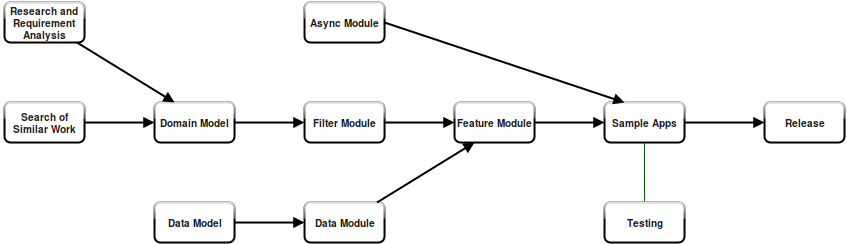
\includegraphics[scale=0.80]{pert.png}
    \newline
    \caption{Pert Diagram}
  \end{figure}
\end{subsection}
\end{landscape}
\newpage
\begin{subsection}{Risk Management}
  \paragraph{}{%
  The development team is unexperienced on computer vision field, so some learning
  period is required in multiple phases of the project. Especially developing modules that contain algorithms
  having steep learning curve will take remarkable time in the process. For this reason it is crucial to comply with
  the schedule.\\
  }
\end{subsection}
\end{section}

\newpage

\begin{section}{Methodology and Analysis}
  \begin{subsection}{Feasibility Study}
    \paragraph{}{reVision is an open source and non-profit project so there is no need to examine the financial feasibility. The project is analyzed only in operational and technical sides.}
    \begin{subsubsection}{Operational Feasibility}
      \paragraph{}{Computer vision developers feel the lack of a decent computer vision library on Android platform. Creating a high performance computer vision application on Android takes too much effort. This project, if succeeds will become a ready-to-use and collaborative tool for Android developers.}
    \end{subsubsection}

    \begin{subsubsection}{Technical Feasibility}
      \paragraph{}{Widely used libraries for computer vision and GPU computing such as OpenCV, OpenCL, and CUDA, cannot be used on Android platform because of incompatibilities of devices and lack of drivers. For this reason a new GPU computing engine named Renderscript was presented. But Renderscript does not have a complete computer vision library.}
      \paragraph{}{reVision uses Renderscript for data-parallel GPU computations. Since Renderscript technology is hardware and version independent among all recent Android devices, reVision can also be used universally on every Android device. The runtime frame-rates vary between different devices but reVision is ensured to work at the most efficient way that the device is capable of.}
    \end{subsubsection}
  \end{subsection}
  \newpage
  \begin{subsection}{The Process Model and Its Particular Adaptation}
    \paragraph{}{According to R. S. Pressman \cite{pressman} there are several process model types including linear sequential model, prototype model, evolutionary models and etc. In real life most them are used according to the project necessities and requirements.}
\paragraph{}{reVision is being developed using incremental model which is an evolutionary model. Every release is published after a work cycle which includes all the phases of the software development process. Each release extends the project with at least one module or functionality with its sample application.}
\paragraph{}{Incremental model is suitable for this project because the project team is not experienced in computer vision field. The incremental model gives the option of refactoring the design and evolving the project through time to the team, which other models would not give.}
\paragraph{}{Development cycle can simply be clarified with following steps; Requirement analysis, Planning, Design, Implementation and Testing. Every development iteration of reVision include each one of those steps.}
  \end{subsection}
  \newpage
  \begin{subsection}{Functional and Non-Functional Requirements}
    \begin{subsubsection}{Functional Requirements}
      \paragraph{Filtering:}{
      Image filtering is required for other modules to provide initial data. It also can be used as standalone to get filtered image.
      }
      \paragraph{Feature Detection:}{
      Feature detection is one of the outputs of the library which provides marked image matrix of the detected features such as edges, corners, blobs.
      }
      \paragraph{Object Tracking:}{
      Object tracking is one of the features of the library which detects the object and tracks the object in the given stream.
      }
      \newline
      \vspace{1cm}
      \newline
      \lstset{language=C++,
                      caption={Harris Kernel from the first prototype},
                      captionpos=b,
                      backgroundcolor=\color{black!5},
                      keywordstyle=\color{new-blue},
                      stringstyle=\color{red},
                      commentstyle=\color{green},
                      basicstyle=\footnotesize,% basic font setting
                      morecomment=[l][\color{magenta}]{\#}
      }
      {\ttfamily
      \begin{lstlisting}
        uchar4 __attribute__((kernel)) harris(const uchar4 in,
          uint32_t x, uint32_t y)
        {
            float c = 0.04;
            float4 convXpixel =
              rsUnpackColor8888(rsGetElementAt_uchar4(convX, x, y));
            float4 convYpixel =
              rsUnpackColor8888(rsGetElementAt_uchar4(convY, x, y));

            float Ix = convXpixel.r * gMonoMult[0] + convXpixel.g *
              gMonoMult[1] + convXpixel.b * gMonoMult[2];
            float Iy = convYpixel.r * gMonoMult[0] + convYpixel.g *
              gMonoMult[1] + convYpixel.b * gMonoMult[2];

            float Ixx = Ix * Ix;
            float Iyy = Iy * Iy;
            float Ixy = Ix * Iy;
            float cornerResponse =
              (Ixx*Iyy - Ixy*Ixy - c*(Ixx+Iyy)*(Ixx+Iyy));

            if(cornerResponse < harrisThreshold ) {
                cornerColorRGB.r = 0;
                cornerColorRGB.g = 255;
                cornerColorRGB.b = 0;
                return cornerColorRGB;
            } else {
                return in;
            }
        }
      \end{lstlisting}
      }
    \end{subsubsection}
    \newpage
    \begin{subsubsection}{Non-Functional Requirements}
      \paragraph{Performance Requirements:}{
      The response time problem were the thing that triggered the creation of reVision project. Without reasonable
      performance, reVision could not be considered successful. To achieve the desired performance, developers implement
      and use all performance related modules such as implementing Async Model or using Renderscript framework. The
      performance is the single most important non-functional requirement of reVision.
      }
      ​
      \paragraph{Reliability Requirements:}{
      The responses of reVision modules must be correct and precise.
      }
      ​
      \paragraph{Usability Requirements:}{ The function arguments and the Android communication modules must be easy
       to understand and to use. Since it is a library, every function has to be well documented. Also the sample
       applications have to be complete and ready to test for users.
      }
    \end{subsubsection}
  \end{subsection}
  \newpage
  \begin{subsection}{Use Cases}
    \begin{tabularx}{\textwidth}{|*{2}{Y|}}
     \hline
     \multicolumn{1}{|l|}{\textbf{Use Case No}} & 1\\
     \hline
     \multicolumn{1}{|l|}{\textbf{Use Case Name}} & Filter Image \\
     \hline
     \multicolumn{1}{|l|}{\textbf{Actor}} & User \\
     \hline
     \multicolumn{1}{|l|}{\textbf{Preconditions}} & Retrieve data in an appropriate way \\
     \hline
     \multicolumn{1}{|l|}{\textbf{Postconditions}} & Return filtered image data \\
     \hline
     \multicolumn{1}{|l|}{\textbf{Scenario}} & User gets filtered image\\
     \hline
   \end{tabularx}
   \newline
   \vspace{1cm}
   \newline
   \begin{tabularx}{\textwidth}{|*{2}{Y|}}
    \hline
    \multicolumn{1}{|l|}{\textbf{Use Case No}} & 2\\
    \hline
    \multicolumn{1}{|l|}{\textbf{Use Case Name}} & Detect Corners with Harris Algorithm \\
    \hline
    \multicolumn{1}{|l|}{\textbf{Actor}} & User \\
    \hline
    \multicolumn{1}{|l|}{\textbf{Preconditions}} & Retrieve data in an appropriate way \\
    \hline
    \multicolumn{1}{|l|}{\textbf{Postconditions}} & Return image with corner data \\
    \hline
    \multicolumn{1}{|l|}{\textbf{Scenario}} & Locate all local maxima of the filtered image, then mark the highest N on the image\\
    \hline
  \end{tabularx}
  \newline
  \vspace{1cm}
  \newline
  \begin{tabularx}{\textwidth}{|*{2}{Y|}}
   \hline
   \multicolumn{1}{|l|}{\textbf{Use Case No}} & 3\\
   \hline
   \multicolumn{1}{|l|}{\textbf{Use Case Name}} & Detect Corners with FAST Algorithm \\
   \hline
   \multicolumn{1}{|l|}{\textbf{Actor}} & User \\
   \hline
   \multicolumn{1}{|l|}{\textbf{Preconditions}} & Retrieve data in an appropriate way \\
   \hline
   \multicolumn{1}{|l|}{\textbf{Postconditions}} & Return image with corner data \\
   \hline
   \multicolumn{1}{|l|}{\textbf{Scenario}} & User gets the image marked by FAST corner detection results\\
   \hline
 \end{tabularx}
 \newpage
  \begin{tabularx}{\textwidth}{|*{2}{Y|}}
       \hline
       \multicolumn{1}{|l|}{\textbf{Use Case No}} & 4 \\
       \hline
       \multicolumn{1}{|l|}{\textbf{Use Case Name}} & Feature matching with SIFT descriptors \\
       \hline
       \multicolumn{1}{|l|}{\textbf{Actor}} & User \\
       \hline
       \multicolumn{1}{|l|}{\textbf{Preconditions}} & Retrieve data in an appropriate way \\
       \hline
       \multicolumn{1}{|l|}{\textbf{Postconditions}} & Return the image back with markers \\
       \hline
       \multicolumn{1}{|l|}{\textbf{Scenario}} & User gets the match of image extracted before \\
       \hline
    \end{tabularx}
    \newline
    \vspace{1cm}
    \newline
    \begin{tabularx}{\textwidth}{|*{2}{Y|}}
          \hline
          \multicolumn{1}{|l|}{\textbf{Use Case No}} & 5 \\
          \hline
          \multicolumn{1}{|l|}{\textbf{Use Case Name}} & Track a specific object \\
          \hline
          \multicolumn{1}{|l|}{\textbf{Actor}} & User \\
          \hline
          \multicolumn{1}{|l|}{\textbf{Preconditions}} & Retrieve data in an appropriate way \\
          \hline
          \multicolumn{1}{|l|}{\textbf{Postconditions}} & Return the image back with an object marker \\
          \hline
          \multicolumn{1}{|l|}{\textbf{Scenario}} & User tracks a specific object \\
          \hline
    \end{tabularx} \\
    \newline
    \vspace{1cm}
    \newline
    \begin{tabularx}{\textwidth}{|*{2}{Y|}}
             \hline
             \multicolumn{1}{|l|}{\textbf{Use Case No}} & 6 \\
             \hline
             \multicolumn{1}{|l|}{\textbf{Use Case Name}} & Understand functionality of the library with sample applications \\
             \hline
             \multicolumn{1}{|l|}{\textbf{Actor}} & User \\
             \hline
             \multicolumn{1}{|l|}{\textbf{Preconditions}} & - \\
             \hline
             \multicolumn{1}{|l|}{\textbf{Postconditions}} & - \\
             \hline
             \multicolumn{1}{|l|}{\textbf{Scenario}} & User understands the functionality of the library with sample applications \\
             \hline
           \end{tabularx}

  \end{subsection}
\end{section}
\newpage
\begin{section}{Planned Solution/Product}
  \paragraph{}{
  reVision is planned to be an open source computer vision library that can operate on all Android devices.
  By using the power of Renderscript, it will provide ready to use computer vision algorithm implementations
  with their sample applications.
  }
  \paragraph{}{
  Computer vision algorithms will be implemented in Renderscript. When the Renderscript was presented, the goal of
  it had been to bring a higher performance API to Android developers \cite{renderscript_release}.
  So, the goal of reVision is to present a higher level, closer to Renderscript performance, and easy-to-use
  API to Android developers.
  }
  \paragraph{}{
  Sample applications are planned to exemplify all features of the library in order to guide the developers on
  their developing process. Figure 1 indicates a couple of pictures from first prototype of reVision. Image on the
  bottom is a Harris Algortihm applied form of the top.

  }
  \begin{figure}[h]
    \centering
    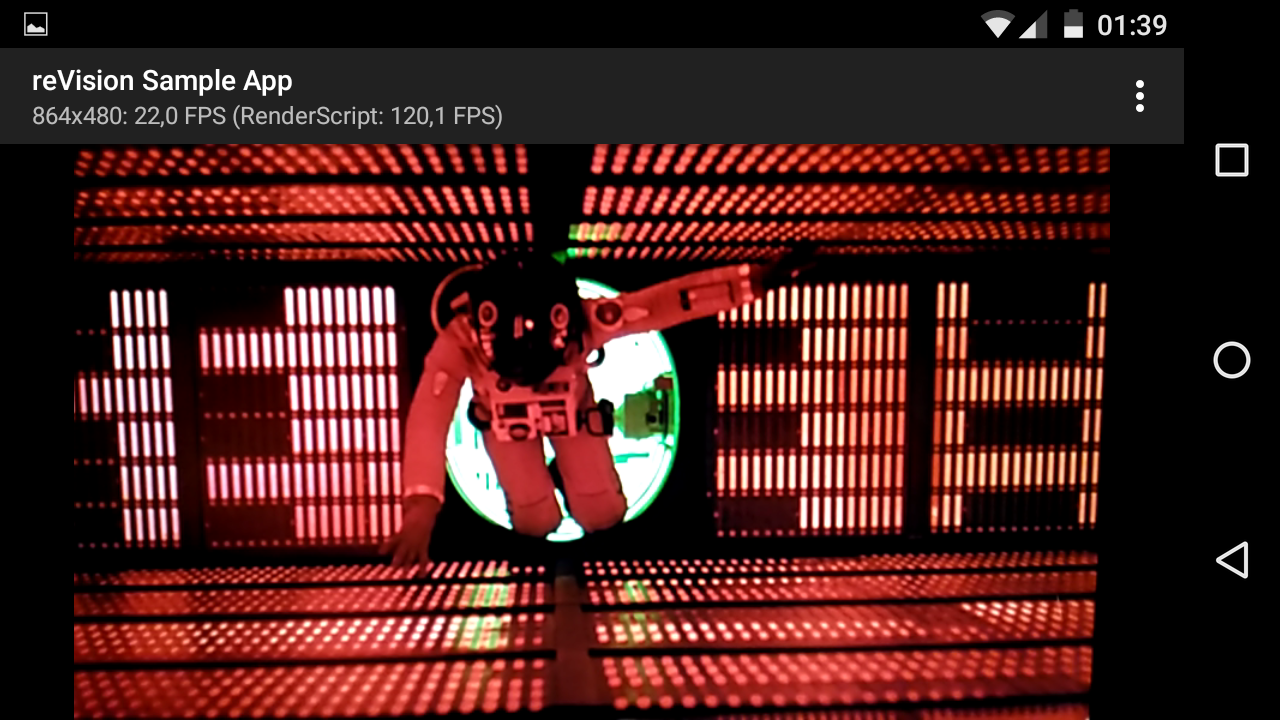
\includegraphics[scale=0.25]{clean.png}
    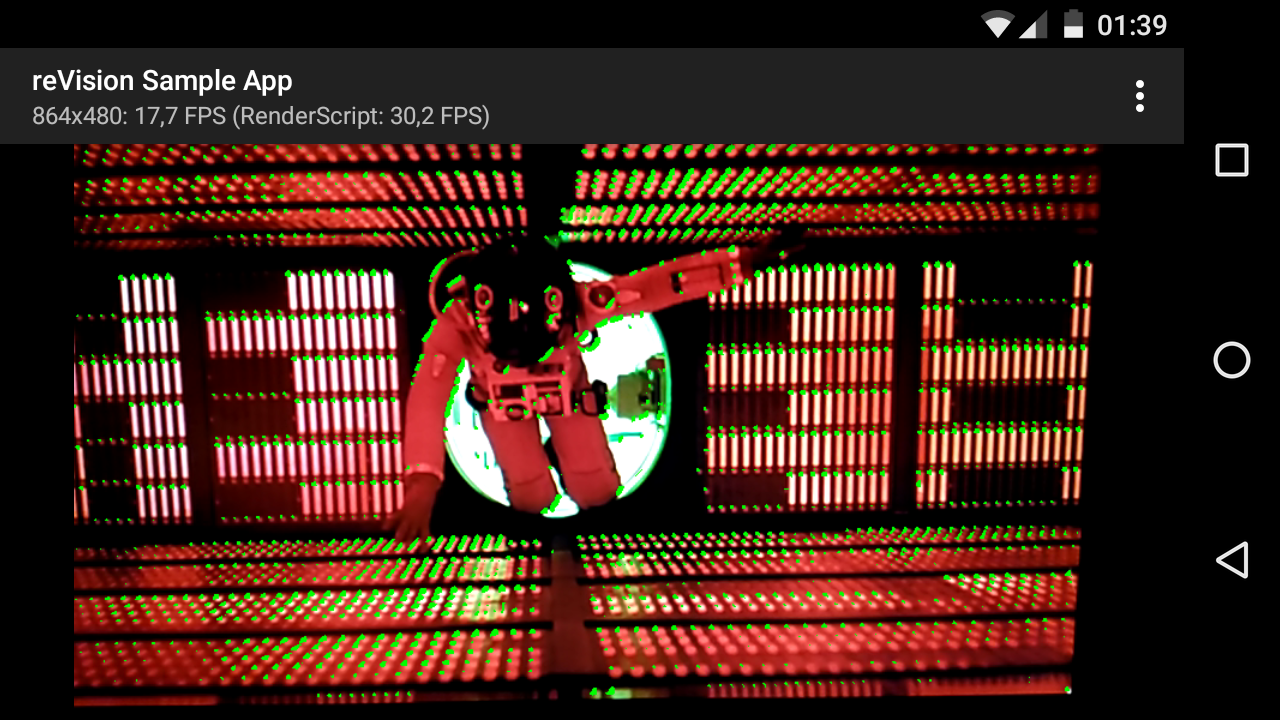
\includegraphics[scale=0.25]{detected.png}

    \caption{First prototype of reVision: Implementation of Harris Corner Detection}
    \label{fig:mesh1}
  \end{figure}


  \paragraph{}{
  Eventually, reVision will be a solution to absence of an easy-to-use, and well performanced library operates on
  all Android devices.
  }

\end{section}
\newpage
\begin{section}{Related Work/Similar Solutions}
\paragraph{}{
  There are several libraries about the vision. One of the most significant of them is OpenCV.
}

  \paragraph{}{
  \begin{wrapfigure}{l}{0.25\textwidth}
    \centering
    
\includegraphics[width=0.25\textwidth]{opencv.png}
\end{wrapfigure}

OpenCV is released under a BSD license and hence it’s free for
both academic and commercial use. It has C++, C, Python and Java interfaces and supports Windows, Linux, Mac OS,
iOS and Android. OpenCV was designed for computational efficiency and with a strong focus on real-time applications.
Written in optimized C/C++, the library can take advantage of multi-core processing. Enabled with OpenCL, it can
take advantage of the hardware acceleration of the underlying heterogeneous compute platform. Adopted all around
the world, OpenCV has more than 47 thousand people of user community and estimated number of downloads exceeding 9
million. Usage ranges from interactive art, to mines inspection, stitching maps on the web or through advanced
robotics \cite{opencv}.

  }

  \paragraph{}{
  \begin{wrapfigure}{r}{0.25\textwidth}
    \centering
    
\includegraphics[width=0.25\textwidth]{fastcv.jpg}
\end{wrapfigure}
Another computer vision library is the Qualcomm's FastCV\textsuperscript{TM} \cite{fastcv}. FastCV\textsuperscript{TM} library offers a
mobile-optimized computer vision (CV) library which includes the most frequently used vision processing functions
for use across a wide array of mobile devices, even mass-market handsets. Middleware developers can use FastCV to
build the frameworks needed by developers of computer vision apps; Qualcomm's Augmented Reality (AR) SDK is a good
example. Developers of advanced CV application can also use FastCV functions directly in their application. FastCV will
enable you to add new user experiences into your camera-based apps like:
\begin{itemize}
  \item gesture recognition
  \item face detection, tracking and recognition
  \item text recognition and tracking
  \item augmented reality
\end{itemize}

}

\paragraph{}{
Also Cuda\textsuperscript{TM} \cite{cuda} can be mentioned as a similar work. CUDA\textsuperscript{TM} is a parallel computing platform and programming model invented by
NVIDIA. It enables dramatic increases in computing performance by harnessing the power of the graphics processing unit
(GPU). To use CUDA on your system, you will need the following:
\begin{itemize}
  \item Android development device with a CUDA-capable GPU
  \item A supported version of Linux to cross-compile
  \item NVIDIA CodeWorks for Android with CUDA support
\end{itemize}
}

\end{section}

\newpage

\begin{section}{Impact}

\paragraph{}{
In the impact section, realistic constraints of the project will be mentioned. Besides being a thesis project,
reVision is a nonprofit project as a matter of course, aims to make the Android world a better place for computer vision
application developers. Thus, there are several constraints about the project. When compared to similar works,
reVision is maintained by students instead of groups of experienced developers or big companies.
So, this situation limits the scope of the project, but it also motivates its participants about the dream of
taking part in a project that can be a milestone as well.

}

\paragraph{}{
  reVision is also an opportunity to learn new technologies and methodologies for its developers. It focuses on the
  computer vision and its applications using mobile devices, and data-parallel GPU computation. So, project team participants
  get a chance to improve themselves in these topics. The project will help the developers to understand the formal procedures
  of writing formal reports. Nearly all the software engineering processes are revisited.
}

\paragraph{}{
  All in all,  reVision is a hardware independent computer vision library with companion sample applications
  for Android which will be an open source and GPU-ready, and strives to make Android developers more productive
  on computer vision projects.

}

\end{section}

\newpage
          \begin{thebibliography}{9}
          \bibitem{renderscript_release}
            Introducing Renderscript -
              http://android-developers.blogspot.com.tr/2011/02/introducing-renderscript.html

          \bibitem{renderscript_api}
            Renderscript - http://developer.android.com/intl/es/guide/topics/renderscript/compute.html

          \bibitem{pressman}
            Roger S. Pressman, Software Engineering A Practitioner's Approach,
            McGraw-Hill, 2001, pp. 26-39

          \bibitem{opencv}
            OpenCV -  http://opencv.org/

          \bibitem{fastcv}
            FastCV - https://developer.qualcomm.com/software/fastcv-sdk

          \bibitem{cuda}
          Cuda - http://docs.nvidia.com/gameworks/content/technologies/mobile/cuda\_android\_main.htm

          \end{thebibliography}

\end{document}
